\section{NTFS}
\subsection{Introducción}
\begin{frame}{Introducción}
  \begin{itemize}
    \item Reemplazo de Microsoft para los sistemas FAT.
    \item Mejoras importantes como soporte de metadatos y uso de estructuras de datos avanzadas.
    \item Debido a que sus especificaciones son secretas no tiene buen soporte en sistemas no Microsoft.
  \end{itemize}
\end{frame}

\subsection{Características}
\begin{frame}{Características}
  \begin{itemize}
    \item Journaling (Solo para la parte de metadatos)
    \item ACLs
    \item Cifrado
    \item Compresion
    \item Tamaño máximo: 16TB
    \item Tamaño máximo de fichero: 16TB
    \item Máximo de caracteres de nombre de fichero: 256B
    \item Máximo número de ficheros: 4.294.967.295
  \end{itemize}
\end{frame}

\subsection{Estructura}
\begin{frame}{Estructura}
  \begin{itemize}
    \item Al principio de la partición nos encontramos el sector de arranque.
    \item Justo después se encuentra la MFT (Master File Table).
    \item Cada entrada del MFT es un fichero del sistema de ficheros.
    \item Las primeras 16 entradas de la MFT son ficheros de metadatos.
    \item Después tenemos el área de datos.
    \item En medio de la partición, aproximadamente, nos encontramos una copia de la MFT
    \item Al final de la partición nos encontramos un backup del sector de arranque.
  \end{itemize}
\end{frame}

\begin{frame}{Estructura}
  \begin{center}
    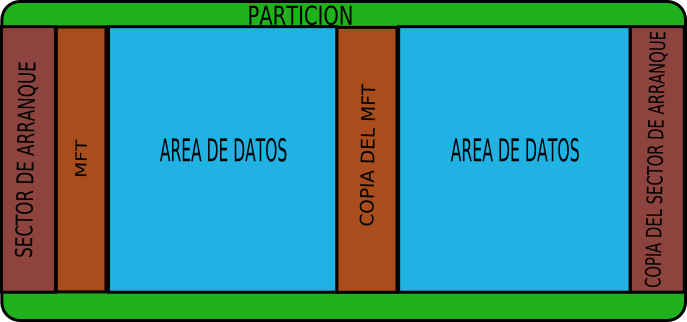
\includegraphics[height=5.5cm]{imgs/ntfs_struct.png}
  \end{center}
\end{frame}

\begin{frame}{Ficheros}
  \begin{itemize}
    \item Los ficheros contienen información sobre el fichero, atributos y características.
    \item Si el fichero es pequeño lo incluye directamente en el MFT
    \item Si el fichero es grande crea va almacenando los datos en "extents" (grupos de clusters fuera del MFT).
    \item Si el fichero fuera tan grande que no cupieran más direcciones de "extents", externalizaría las direcciones.
    \item De este modo seguiría creciendo hasta que no se necesite más espacio.
    \item Los directorios contiene los ficheros ordenados a modo de arbol B.
  \end{itemize}
\end{frame}

\begin{frame}{Ficheros}
  \begin{center}
    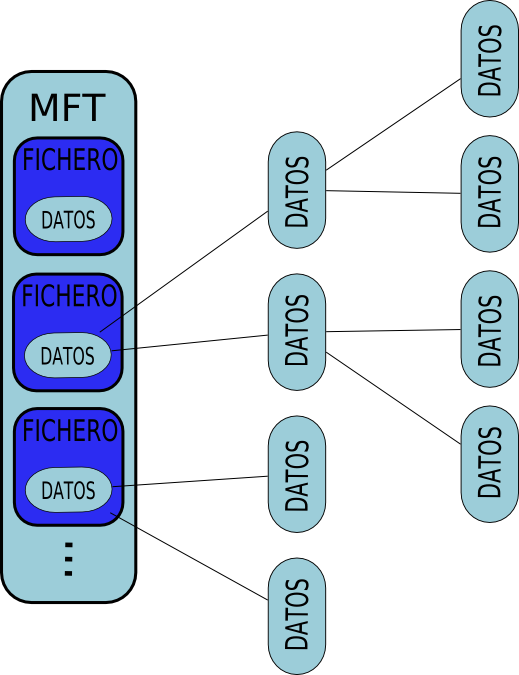
\includegraphics[height=6cm]{imgs/ntfs_files.png}
  \end{center}
\end{frame}
